%% For double-blind review submission, w/o CCS and ACM Reference (max submission space)
\documentclass[sigplan,10pt,review,anonymous]{acmart}\settopmatter{printfolios=true,printccs=false,printacmref=false}
%% For double-blind review submission, w/ CCS and ACM Reference
%\documentclass[sigplan,10pt,review,anonymous]{acmart}\settopmatter{printfolios=true}
%% For single-blind review submission, w/o CCS and ACM Reference (max submission space)
%\documentclass[sigplan,10pt,review]{acmart}\settopmatter{printfolios=true,printccs=false,printacmref=false}
%% For single-blind review submission, w/ CCS and ACM Reference
%\documentclass[sigplan,10pt,review]{acmart}\settopmatter{printfolios=true}
%% For final camera-ready submission, w/ required CCS and ACM Reference
%\documentclass[sigplan,10pt]{acmart}\settopmatter{}


%% Conference information
%% Supplied to authors by publisher for camera-ready submission;
%% use defaults for review submission.
\acmConference[PL'17]{ACM SIGPLAN Conference on Programming Languages}{January 01--03, 2017}{New York, NY, USA}
\acmYear{2017}
\acmISBN{} % \acmISBN{978-x-xxxx-xxxx-x/YY/MM}
\acmDOI{} % \acmDOI{10.1145/nnnnnnn.nnnnnnn}
\startPage{1}

%% Copyright information
%% Supplied to authors (based on authors' rights management selection;
%% see authors.acm.org) by publisher for camera-ready submission;
%% use 'none' for review submission.
\setcopyright{none}
%\setcopyright{acmcopyright}
%\setcopyright{acmlicensed}
%\setcopyright{rightsretained}
%\copyrightyear{2017}           %% If different from \acmYear

%% Bibliography style
\bibliographystyle{ACM-Reference-Format}
%% Citation style
%\citestyle{acmauthoryear}  %% For author/year citations
%\citestyle{acmnumeric}     %% For numeric citations
%\setcitestyle{nosort}      %% With 'acmnumeric', to disable automatic
                            %% sorting of references within a single citation;
                            %% e.g., \cite{Smith99,Carpenter05,Baker12}
                            %% rendered as [14,5,2] rather than [2,5,14].
%\setcitesyle{nocompress}   %% With 'acmnumeric', to disable automatic
                            %% compression of sequential references within a
                            %% single citation;
                            %% e.g., \cite{Baker12,Baker14,Baker16}
                            %% rendered as [2,3,4] rather than [2-4].


%%%%%%%%%%%%%%%%%%%%%%%%%%%%%%%%%%%%%%%%%%%%%%%%%%%%%%%%%%%%%%%%%%%%%%
%% Note: Authors migrating a paper from traditional SIGPLAN
%% proceedings format to PACMPL format must update the
%% '\documentclass' and topmatter commands above; see
%% 'acmart-pacmpl-template.tex'.
%%%%%%%%%%%%%%%%%%%%%%%%%%%%%%%%%%%%%%%%%%%%%%%%%%%%%%%%%%%%%%%%%%%%%%


%% Some recommended packages.
\usepackage{booktabs}   %% For formal tables:
                        %% http://ctan.org/pkg/booktabs
\usepackage{subcaption} %% For complex figures with subfigures/subcaptions
                        %% http://ctan.org/pkg/subcaption

\usepackage{xspace}
\newcommand{\CEU}{\textsc{C\'{e}u}\xspace}

\begin{document}

%% Title information
\title{Where Do Events Come From?}
\subtitle{Reactive Programming From The Ground Up}

%% Author information
%% Contents and number of authors suppressed with 'anonymous'.
%% Each author should be introduced by \author, followed by
%% \authornote (optional), \orcid (optional), \affiliation, and
%% \email.
%% An author may have multiple affiliations and/or emails; repeat the
%% appropriate command.
%% Many elements are not rendered, but should be provided for metadata
%% extraction tools.

%% Author with single affiliation.
\author{First1 Last1}
\authornote{with author1 note}          %% \authornote is optional;
                                        %% can be repeated if necessary
\orcid{nnnn-nnnn-nnnn-nnnn}             %% \orcid is optional
\affiliation{
  \position{Position1}
  \department{Department1}              %% \department is recommended
  \institution{Institution1}            %% \institution is required
  \streetaddress{Street1 Address1}
  \city{City1}
  \state{State1}
  \postcode{Post-Code1}
  \country{Country1}                    %% \country is recommended
}
\email{first1.last1@inst1.edu}          %% \email is recommended

%% Author with two affiliations and emails.
\author{First2 Last2}
\authornote{with author2 note}          %% \authornote is optional;
                                        %% can be repeated if necessary
\orcid{nnnn-nnnn-nnnn-nnnn}             %% \orcid is optional
\affiliation{
  \position{Position2a}
  \department{Department2a}             %% \department is recommended
  \institution{Institution2a}           %% \institution is required
  \streetaddress{Street2a Address2a}
  \city{City2a}
  \state{State2a}
  \postcode{Post-Code2a}
  \country{Country2a}                   %% \country is recommended
}
\email{first2.last2@inst2a.com}         %% \email is recommended
\affiliation{
  \position{Position2b}
  \department{Department2b}             %% \department is recommended
  \institution{Institution2b}           %% \institution is required
  \streetaddress{Street3b Address2b}
  \city{City2b}
  \state{State2b}
  \postcode{Post-Code2b}
  \country{Country2b}                   %% \country is recommended
}
\email{first2.last2@inst2b.org}         %% \email is recommended


%% Abstract
%% Note: \begin{abstract}...\end{abstract} environment must come
%% before \maketitle command

\begin{abstract}
In reactive and event-based systems, execution is guided by an external
environment which generates inputs to the application and consumes outputs from
it.
Reactive languages provide dedicated syntax and semantics to deal with events
and greatly simplify the programming experience in this domain.
%
Nevertheless, the environment is typically prefabricated in a host language and
the very central concept of events is implemented externally to the reactive
language.
%
In this work, we propose an interrupt handler primitive for a reactive language
targeting embedded systems in order to take control of the whole event loop,
from a sensor input source and back to an actuator output.
%
We propose the new primitive in the context of the structured reactive language
\CEU and discuss they synergize to provide automatic standby for applications
and hot swapping of device drivers, while avoiding race conditions.
\end{abstract}

%% 2012 ACM Computing Classification System (CSS) concepts
%% Generate at 'http://dl.acm.org/ccs/ccs.cfm'.
\begin{CCSXML}
<ccs2012>
<concept>
<concept_id>10011007.10011006.10011008</concept_id>
<concept_desc>Software and its engineering~General programming languages</concept_desc>
<concept_significance>500</concept_significance>
</concept>
<concept>
<concept_id>10003456.10003457.10003521.10003525</concept_id>
<concept_desc>Social and professional topics~History of programming languages</concept_desc>
<concept_significance>300</concept_significance>
</concept>
</ccs2012>
\end{CCSXML}

\ccsdesc[500]{Software and its engineering~General programming languages}
\ccsdesc[300]{Social and professional topics~History of programming languages}
%% End of generated code


%% Keywords
%% comma separated list
\keywords{interrupt service routine,
          sleep mode,
          synchronous reactive programming}

\maketitle

\section{Introduction}

Reactive applications interact continuously and in real time with the external
world through sensors and actuators (e.g., buttons, displays, timers, etc.).
%
These interactions are typically represented as input events flowing from the
devices to the application and as output events flowing from the application to
the devices.
%
As illustrated in Figure~\ref{fig.loop}, devices can be encapsulated as a
single component, \emph{the environment}, which controls the system execution
in an event loop:
the application sits idle waiting for an input;
the environment awakes the application on the occurrence of an input;
the application reacts to the input and generates back one or more outputs;
the application becomes idle and the loop restarts.

\begin{figure}
\centering
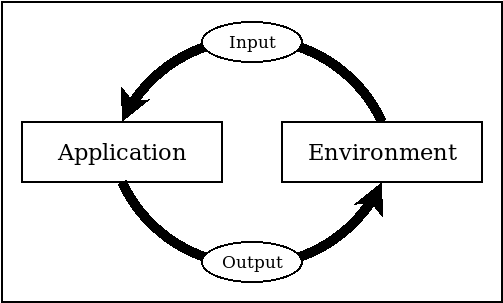
\includegraphics[width=\linewidth]{loop}
\caption{ Event loop in reactive systems.
          The environment controls the application through input \& output
          events.
\label{fig.loop}
}
\end{figure}

The environment is typically implemented in a host language (e.g., C) and
controls the main event loop, invoking entry points in the reactive language
runtime on the occurrence of inputs and also receiving output calls, both
through a documented API.
%
As examples, Esterel~\cite{esterel.ieee91} relies on C for passing events
between the environment and the running program~\cite{esterel.book.compiling},
while Elm~\cite{frp.elm} uses the concept of \emph{ports}, which allows sending
out values to JavaScript in commands and listening for values in
subscriptions~\cite{frp.elm.ports}.

%This separation exposes the environment as a rigid system component that
%evolves in separate from the application.
The event-based separation between the application and the environment is
arguably inevitable and also happens at the right level of abstraction, since
it connects the application with the operating system resources through a
non-invasive API.
%
However, it involves two languages and the programmer may have to deal with
multiple syntaxes, incompatible type systems, and different address spaces.
%
Furthermore, in the context of embedded systems, a proper host OS may even be
absent or lacking enough device drivers, which requires more low-level
intervention from the application.

In this work, we propose
an interrupt handler primitive for a reactive language in
order to take control of the whole event loop, from the
hardware input source and back to the hardware output
sink. We propose the new primitive in the context of
the structured reactive language \CEU and discuss how
it synergizes with the structured paradigm to provide
automatic standby for applications and hot swapping
for drivers during runtime.

We present two uses cases that take advantage of the tight integration between
the language and environment:


with different syntaxes and semantics.
For instance, , type systems, and



abstraction
    - rigid
    - two languages
        - syntax and semantics
            - integrates with features such as lexical scope, type system
    - platforms w/o OS

\newpage

\begin{figure}
\centering
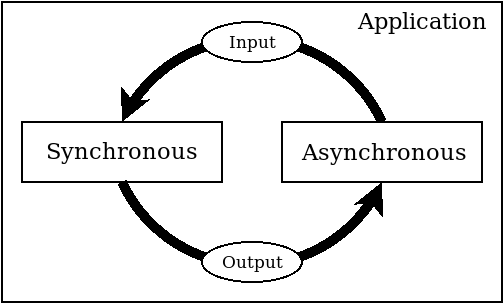
\includegraphics[width=\linewidth]{sync-async}
\caption{ Event loop in reactive systems.
          The environment controls the application through input \& output
          events.
\label{fig.loop}
}
\end{figure}

what would be

output (int,int) O;

becomes

output (int x, int y) O do
end

\begin{comment}
% Esterel
https://books.google.com.br/books?id=O5zi14i0KP4C&pg=PA31&lpg=PA31&dq=esterel+external+signal+api&source=bl&ots=43EBAqIkSJ&sig=npYylZteOmZAqv4f7SXAtJO9xr8&hl=en&sa=X&ved=0ahUKEwjFlf7-3p_cAhWPrVkKHXsFDWgQ6AEIUjAG#v=onepage&q=esterel%20external%20signal%20api&f=false
Esterel relies on general-purpose languages such as C or C++ in two ways.       
First, for portability, most Esterel compilers generate C instead of            
assembly or some other executable representation.                               
Such generated code provides an interface for passing events between the        
environment and the running program.                                            
Second, Esterel allows the use of data types and functions defined externally   
(e.g., in C) to be used within an Esterel program.                              

% Elm
https://guide.elm-lang.org/interop/javascript.html
Okay, in Elm, any communication with JavaScript goes through a port. Think of
it like a hole in the side of your Elm program where you can send values in and
out. These work exactly like the commands and subscriptions from the
Architecture section. Sending values out to JS is a command. Listening for
values coming in from JS is a subscription. Pretty neat!
\end{comment}

- excel define formulas for input but not the input itself

output -> input

the environment sits
    inverse
    reacts to output and generates inputs

remain idle and react to the occurrence of events 


%% Acknowledgments
\begin{acks}                            %% acks environment is optional
                                        %% contents suppressed with 'anonymous'
  %% Commands \grantsponsor{<sponsorID>}{<name>}{<url>} and
  %% \grantnum[<url>]{<sponsorID>}{<number>} should be used to
  %% acknowledge financial support and will be used by metadata
  %% extraction tools.
  This material is based upon work supported by the
  \grantsponsor{GS100000001}{National Science
    Foundation}{http://dx.doi.org/10.13039/100000001} under Grant
  No.~\grantnum{GS100000001}{nnnnnnn} and Grant
  No.~\grantnum{GS100000001}{mmmmmmm}.  Any opinions, findings, and
  conclusions or recommendations expressed in this material are those
  of the author and do not necessarily reflect the views of the
  National Science Foundation.
\end{acks}


%% Bibliography
\bibliography{my,other}


%% Appendix
\appendix
\section{Appendix}

Text of appendix \ldots

\end{document}
